

%\documentclass[a4paper]{jarticle}


\section{mgpmetis.rb グラフ分割コマンド\label{sect:mgpmetis}}
\index{mgpmetis@mgpmetis}
本コマンドは、ミネソタ大学で開発されたグラフ分割ソフトウェアMETIS
(\url{http://glaros.dtc.umn.edu/gkhome/metis/metis/overview})
を利用しやすいように作成されたコマンドである。
METISによるグラフ分割では、与えられた無向グラフについて、
各パーティション(以下クラスタとも呼ぶ)に含まれる節点数をできるだけ同じにして、
枝のカット数を最小化するように複数のパーティションに分割する。

METISが直接扱うデータ構造は、節点を整数で表したフォーマットであるが、本コマンドでは任意の文字列を扱うことができる。
またグラフデータは、特殊なフォーマットを仮定せず、枝データと節点データを別々にCSVデータとして与える。
内部では、gpmetisコマンドをコールしており、前処理として、ユーザが与えたグラフデータをgpmetisが扱えるデータに変換している。
データ変換だけを実行することも可能である。

入力データは,表\ref{tbl:mgpmetis_inp1}に示されるように、一行が一つの枝を表す節点ペアとして与えられたCSVファイルである。
孤立した節点がなく、節点の重み(後述)を指定しない場合は枝データのみ与えればよい。
対応するグラフが図\ref{fig:mgpmetis_graph}に示されている。
このグラフを2分割したければ、以下のようにコマンドを実行すればよい。

\begin{verbatim}
$ mgpmetis.rb kway=2 ef=node1,node2 ptype=rb ei=input.csv o=output.csv
\end{verbatim}

結果として、表\ref{tbl:mgpmetis_result}に示されるように、
節点名とその節点が属するクラスタ番号が出力される。
図\ref{fig:mgpmetis_gcut}には、最小本数の枝をカットして2分割されている様子が示されている。

\begin{table}[htbp]
\begin{center}
\begin{tabular}{ll}

\begin{minipage}{0.4\hsize}
\begin{center}
\caption{入力データ(input.csv)\label{tbl:mgpmetis_inp1}}
{\small
\begin{tabular}{cc}
\hline
node1&node2\\
\hline
a&b\\
a&c\\
a&e\\
b&c\\
b&d\\
c&d\\
c&e\\
d&f\\
d&g\\
e&f\\
f&g\\
\hline
\end{tabular} 
}
\end{center}
\end{minipage}

\begin{minipage}{0.4\hsize}
\begin{center}
\caption{分割結果データ(output.csv)\label{tbl:mgpmetis_result}}
{\small
\begin{tabular}{crc}
\hline
node&cluster \\
\hline
a&1 \\
b&1 \\
c&1 \\
d&0 \\
e&1 \\
f&0 \\
g&0 \\
\hline
\end{tabular} 
}
\end{center}
\end{minipage}

\end{tabular} 
\end{center}
\end{table} 

\begin{figure}[htbp]
\begin{center}
\begin{tabular}{cc}

\begin{minipage}{0.3\hsize}
\begin{center}
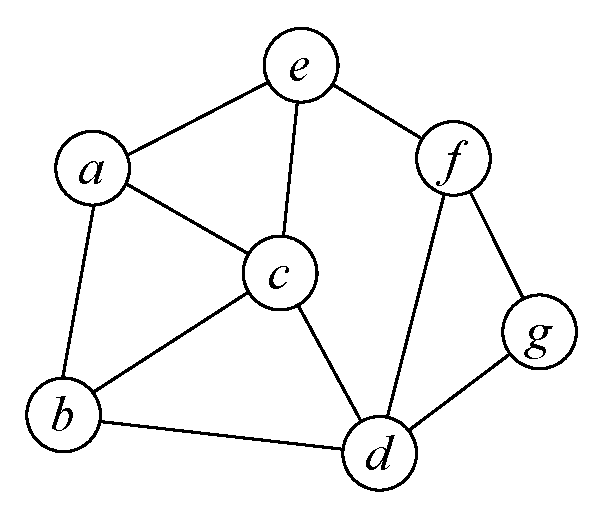
\includegraphics[scale=0.5]{./metis_inpg.eps}
\caption{分割対象のグラフ\label{fig:mgpmetis_graph}}
\end{center}
\end{minipage}

\begin{minipage}{0.7\hsize}
\begin{center}
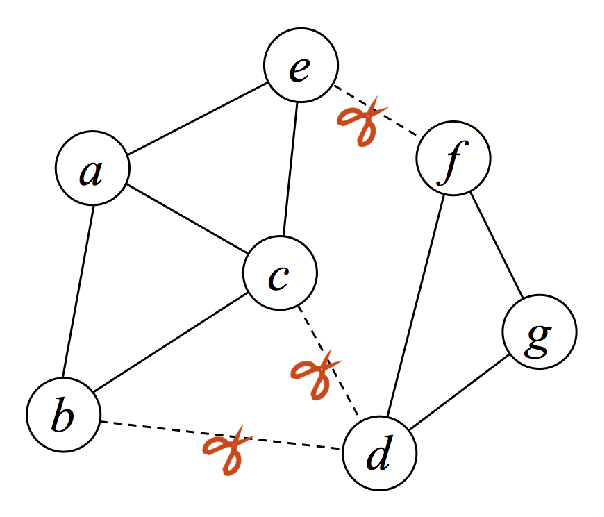
\includegraphics[scale=0.5]{./metis_gcut.eps}
\caption{最小カットによる2分割の結果。
7つの節点があるので、最も均等に分割したとして4:3の分割になるが、
図に示された3つの枝をカットするのが最もカット数が少ないカット方法である。\label{fig:mgpmetis_gcut}}
\end{center}
\end{minipage}

\end{tabular} 
\end{center}
\end{figure} 


\subsection{書式}
\begin{verbatim}
mgpmetis.rb kway= [ptype=rb|kway] ei= [ef=] [ew=] [ni=] [nf=] [nw=] [o=]
            [balance=] [ncuts=] [dat=] [map=] [-noexe] [--help]
\end{verbatim}

\begin{table}[htbp]
{\small
\begin{tabular}{ll}
\verb|ei=|    & : 枝ファイル名(節点ペア)【必須】 \\
\verb|ef=|    & : 枝ファイル上の節点ペア項目名(2項目のみ)【デフォルト:"node1,node2"】 \\
\verb|ew=|    & : 枝ファイル上の重み項目名(1項目のみ)【オプション:省略時は全ての枝の重みを1と見なす】 \\
              & : 重みは整数で指定しなければならない。 \\
\verb|ni=|    & : 節点ファイル名【オプション】 \\
\verb|nf=|    & : 節点ファイル上の節点項目名(1項目のみ)【デフォルト:"node"】 \\
\verb|nw=|    & : 節点ファイル上の重み項目名(複数項目指定可)【オプション:省略時は全ての重みを1と見なす】 \\
              & : 重みは整数で指定しなければならない。 \\
\verb|o=|     & : 出力ファイル名【オプション:defaultは標準出力】 \\
\verb|kway=|  & : 分割数【必須】 \\
\verb|ptype=| & : 分割アルゴリズム【デフォルト:kway】 \\
\verb|balance=| & : パーティション一様化パラメータ【デフォルト: ptype=rbの時は1.001、ptype=kwayの時は1.03】 \\
              & : 式\ref{eq:gpmetis_problem2}における$\beta$の値を指定する。 \\
%\verb|ufactor=| & : 分割アンバランスファクタ【デフォルト: ptype=rbの時は1、ptype=kwayの時は30】 \\
%                & : 式\ref{eq:gpmetis_problem2}における$(\alpha-1)*1000$の値を指定する。 \\
%                & : ex. $\alpha=1.5$に設定したければ、ufactor=500($(1.5-1)*1000$)と指定する。\\
\verb|ncuts=| & : 分割フェーズで、初期値を変えて試行する回数【オプション:default=1】\\

\verb|dat=|   & : 指定されたファイルにgpmetisコマンド用のデータを出力する。 \\
\verb|map=|   & : 指定されたファイルにgpmetisコマンド用の節点番号とi=上の節点名のマッピングデータを出力する。 \\
\verb|-noexe| & : 内部でgpmetisを実行しない。dat=,map=の出力だけが必要な場合に指定する。\\


%\verb|params| & : gpmetisに直接渡すパラメータ文字列を指定する。\\
%              & : ノーチェックで渡されるので、内容を理解して利用する。\\
%              & : 本コマンドで固定されているパラメータもあるため、指定できるパラメータについては注を参照のこと。\\
\verb|--help| & : ヘルプの表示 \\

\end{tabular} 
}
\end{table} 

%\subsubsection{注}
%\verb|params=|で指定できるパラメータは以下の通り。詳細はアルゴリズムの節を参照のこと。
%\begin{table}[htbp]
%{\small
%\begin{tabular}{ll}
%\verb|-ptype=kway|  & 分割方法をk-分割法に切り替える。\\
%                    & 内部では再帰2分割法(-ptype=rb)に固定しているので、その方法を変更できる。\\
%                    & gpmetisコマンドのデフォルトは\verb|kway|であるが、本コマンドでは\verb|rb|としている。\\
%\verb|-iptype=|     & 再帰2分割法における、分割アルゴリズムを指定する。\\
%                    & \verb|nw=|を複数項目指定した場合\verb|grow|が、複数指定した場合は\verb|random|がデフォルトとなる。 \\
%                    & \verb|grow|: GGGP(Greedy Graph Growing Patitioning Algorithm) \\
%                    & \verb|random|: GGP(Graph Grawing Patitioning Algorithm) \\
%\end{tabular} 
%}
%\end{table} 


\subsection{アルゴリズム}
gpmetisによるグラフ分割アルゴリズムは、1)粗化(coarsening)、2)分割(partioning)、3)逆粗化(uncoarsening)の3つのプロセスに分けることができる。
粗化においては、枝で接続された複数の節点を統合する過程で、数百の節点から構成される小さなグラフに縮約するプロセスである。
そして粗化されたグラフについて、
できるだけパーティションサイズを均等にして(統合された節点数を考慮に入れて)、
枝のカット数が最小となるように分割する。
そして最後に、統合された節点を元に戻す逆粗化によって全節点を分割することになる\ref{fig:mgpmetis_abst}。

gpmetisのアルゴリズムの特徴は以下のとおりである。
グラフ分割問題はNP完全であることが知られており、グラフサイズが大きくなると求解が困難となる。
そこで、gpmetisは、前処理でグラフサイズを小さくする粗化によってこの問題を回避している。
しかし、粗化することで分割の自由度が小さくなるため、一般的には分割精度(後述の目的関数により定義される枝カット最小化基準)が悪くなる。
そこで逆粗化の過程で局所の分割構造を改善する(refinement)ことで粗化に伴う精度の悪化を補う。
gpmetisで採用されているアルゴリズムは近似アルゴリズムであり、最適解が得られる保証はないことに注意する。

\begin{figure}[htbp]
\begin{center}
\begin{tabular}{cc}

\begin{minipage}{1.0\hsize}
\begin{center}
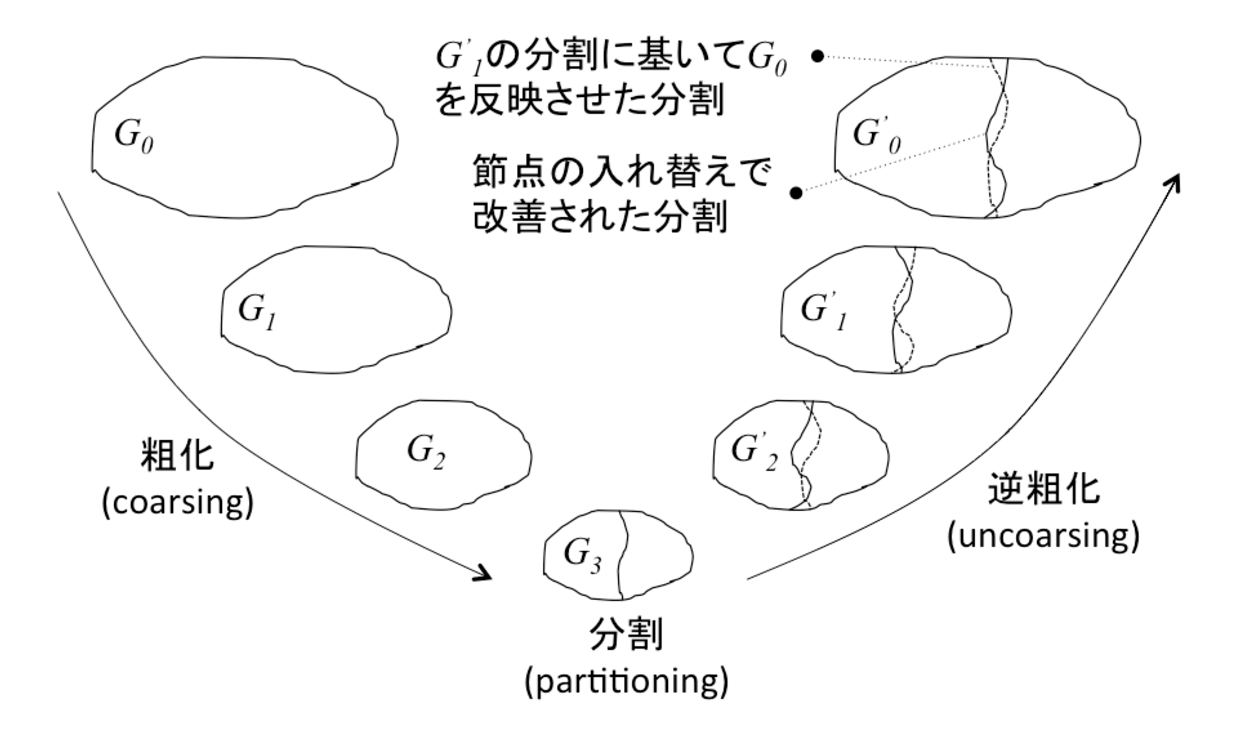
\includegraphics[scale=0.5]{./mgpmetis_abst.eps}
\caption{マルチレベルグラフ分割の概念図(文献\cite{Karypis1999}のFigure1を編集)。
粗化の過程では、節点数が数百になるまで、
グラフマッチングに基づいて節点を併合することで
オリジナルグラフを縮約していく。
縮約されたグラフに対して、節点数をできるだけ一様にして、枝のカット数を最小化するような分割を見つける。
そして、逆粗化の過程で、併合された節点を元に戻していく。
その際、パーティション間で節点の入れ替えを行うことで、最小カットを改善する。
図中、$G_2$と$G'_2$では、構成される節点集合は同じであるが、分割のためにカットされた枝集合が異なる。
\label{fig:mgpmetis_abst}}
\end{center}
\end{minipage}

\end{tabular} 
\end{center}
\end{figure} 



\subsubsection{問題設定}
無向グラフ$G=(V,E)$について、節点集合$V$を$k$個のパーティション$V_1,V_2,\dots,V_k$に分割したい。
%($V_i\cap V_j=\phi(i\ne j),\bigcup_i V_i=V$)。
この時、パーティションをまたいだ枝数を最小化(枝カット最小化)し、
かつ各パーティションに属する節点の数をできるだけ一様にした分割を考える。
より一般的に、頂点$u,v$に張られた枝$(u,v)\in E$の重みを$w(u,v)\ge 0$、
節点$v$に与えられた重みを$w_v$で表すと、
枝カット最小化の目的関数は、式\ref{eq:gpmetis_problem1}の通り定式化できる。
また、パーティションの一様性は、一様化パラメータ$\beta\ge 1.0$を導入した制約条件として定式化される(式\ref{eq:gpmetis_problem2})。
一様化は、パーティションあたりの平均節点数(重み)に対する、最大節点数(重み)の比として定義され、
$\beta$を大きくすれば、よりアンバランスな分割が許容される。
なお、$\beta$はコマンドパラメータ\verb|balance=|で指定できる。

%すなわち2つの目的関数をもつ問題として定式化する。
%より一般的に、頂点$u,v$に張られた枝$(u,v)\in E$の重みを$w(u,v)\ge 0$、
%節点$v$に与えられた重みを$w_v$で表すと、
%それぞれの目的関数は、式\ref{eq:gpmetis_problem1},\ref{eq:gpmetis_problem2}として定式化できる。
%また、一様の基準についてもより一般的に、節点$v$に与えられた重み$w_v$の合計を各パーティションで一様にすることを考える。
%ただし、一般に完全に一様にすることは難しいので、一様化パラメータ$\beta$を導入し、
%式\ref{eq:gpmetis_const}を満たす制約の元で式\ref{eq:gpmetis_problem}を最小化する。

{\footnotesize
\begin{equation}
\argmin_{V_1,V_2,\dots,V_k} \sum_{(u,v)\in E \wedge u\in V_i \wedge v\in V_j \wedge i\ne j} w(u,v) \\
\label{eq:gpmetis_problem1}
\end{equation}
}

{\footnotesize
\begin{equation}
\textrm{subject to}\ \ \frac{\max_i \sum_{v\in V_i} w_v}{\frac{1}{k} \sum_{i=1}^k \sum_{v\in V_i} w_v} \le \beta
\label{eq:gpmetis_problem2}
\end{equation}
}

%{\footnotesize
%\begin{equation}
%\argmin_{V_1,V_2,\dots,V_k} \frac{\max_i \sum_{v\in V_i} w_v}{\frac{1}{k} \sum_{i=1}^k \sum_{v\in V_i} w_v}
%\label{eq:gpmetis_problem2}
%\end{equation}
%}


%以上の多目的問題に対して、パレート解を列挙することも可能ではあるが、
%gpmetisでは、計算効率を優先させ、
%上記の2つの目的をできる限り達成するような分割を、以下で解説するアルゴリズムとして定義している。
%アルゴリズムの詳細についていは\cite{Karypis1999}を参照されたい。

%原著においては、特に以下の様な定式化は示されていない。
%目的関数のみならず、制約条件も満たさない近似解を出力することがある。
%グラフ分割問題にアルゴリズムにより定義したものと考える。

%以下、gpmetisの分割アルゴリズムを示すが、より詳細については\cite{}を参照されたい。

\subsubsection{再帰二分割法とk-Way分割法}
gpmetisが採用しているアルゴリズムの特徴は、NP完全であるグラフ分割問題に対して、
最適解を求めるのではなく、
マルチレベル分割法(multi-level patitioning)を採用することで、
グラフサイズが大きくなっても現実的な時間で計算できるようにしていることにある。
マルチレベル分割法とは、次のような複数のフェーズにより構成されるアルゴリズムの一般的呼称である。
すなわち、オリジナルのグラフを縮約(以下「粗化(Coarsing)」と呼ぶ)することで、
十分に小さいサイズにしてからグラフ分割を実施し、その後、分割精度(枝カット最小化)を改善させながら
粗化グラフを元のサイズのグラフに戻していく(以下「逆粗化(Uncoarsing)」と呼ぶ)。

gpmetisコマンドには、異なる2つの分割アルゴリズム、
マルチレベル再帰二分割法(multi-level recursive bisectioning)と
マルチレベルk-way分割法(multi-level k-way partitioning)が実装されている。
%\footnote{再帰二分割法はpmetis、k-way分割法はkmetisというAPIとして実装されている}。
節点集合$V$を$k$分割する時、再帰二分割方では、オリジナルのグラフを「粗化、分割、逆粗化」によって2分割し、
それぞれのパーティションを更に再帰的に分割していく
\footnote{
再帰分割法では$k$が2のべき乗でなくても、
パーティションの重みを計画的にアンバランスにすることで、
全体としてバランスのとれた分割が可能となる。
例えば、$|V|=9, k=3$であれば、最初の二分割で3:6に分割し、そして6のグラフを再帰的に3:3に分割すればよい。
ただし、Algorithm\ref{algo:mgpmetis_1}では、その詳細は示していない。
}。
再帰二分割法をAlgorithm\ref{algo:mgpmetis_1}に示す。
一方でk-way分割法では、粗化した後にそのグラフを直接$k$分割し、そして逆粗化して終了する。
k-way分割法をAlgorithm\ref{algo:mgpmetis_2}に示す。
いずれか一方が常に優れた分割となるということはないが、
実行時間については、再帰的な分割を行わないためk-way分割法の方が優れている\footnote{
$k=256$で概ね3〜4倍高速との報告がある\cite{Karypis1998}。}
。

\begin{algorithm}
\caption{k分割グラフ分割アルゴリズム:\ \textbf{再帰二分割法}\label{algo:mgpmetis_1}}
\begin{small}
\begin{algorithmic}[1]
\Function{Bisect}{$G,P$}
	\State $G:分割対象グラフ, P: パーティション集合$
 	\If{$G$ のサイズが$1/k$}
		\State $P=P\cup \{G$\} 
	\Else
		\State $C$=Coarsen($G$) \Comment 粗化
		\State $C_1,C_2$ = 2wayPartition($C$) \Comment 粗化グラフを2分割する
		\State $G_1,G_2$ = Uncoarsen($C_1,C_2$) \Comment 逆粗化
		\State $P$=\textsc{Bisect}($G_1,P$) \Comment $G_1$で再帰呼び出し
		\State $P$=\textsc{Bisect}($G_2,P$) \Comment $G_2$で再帰呼び出し
	\EndIf
	\State {\bf return}\ $P$
\EndFunction
\end{algorithmic}
\end{small}
\end{algorithm}

\begin{algorithm}
\caption{k分割グラフ分割アルゴリズム:\ \textbf{$k$-way分割法}\label{algo:mgpmetis_2}}
\begin{small}
\begin{algorithmic}[1]
\Function{Kway}{$G$}
	\State $G:分割対象グラフ$
	\State $C$=Coarsen($G$) \Comment 粗化
	\State $C_1,C_2,\dots,C_k$ = KwayPartition($C$) \Comment 粗化グラフをk分割する
	\State $G_1,G_2,\dots,G_k$ = UncoarsenKway(\{$C_1,C_2,\dots,C_k$\}) \Comment k分割そのまま逆粗化
	\State {\bf return}\ \{$G_1,G_2,\dots,G_k$\}
\EndFunction
\end{algorithmic}
\end{small}
\end{algorithm}

以下では、Algorithm\ref{algo:mgpmetis_1},\ref{algo:mgpmetis_2}に示された各サブ関数、
Coarsen()、2WayPartition()、KwayPartition()、Uncoarsen()、UncoarsenKway()について、以下でその概要のみを示しておく。
詳細についていは\cite{Karypis1999}を参照されたい。

\subsubsection{粗化(Coarsen関数)}
粗化の目的は、分割を効率的に行うためにグラフのサイズを小さくすることである。
%大雑把に言えば、枝で接続された2つの節点を適当に(ランダム)に併合していく。
粗化のアルゴリズムは、再帰二分割法、k-way分割法で共通である。
粗化においては、オリジナルグラフ$G_0=(V_0,E_0)$から、極大マッチング$M$を求め%(計算方法は後述)、
そのマッチングの各要素(枝)を併合して新たな節点とすることで、新たなグラフ$G_1=(V_1,E_1)$を生成する。
ここで、グラフ$G=(V,E)$におけるマッチング$M$とは、枝集合$E$の部分集合で($M \subseteq E$)、
任意の2つの枝$e_1,e_2 \in M$が頂点をお互いに共有しないような枝集合のことである。
そして、マッチング$M$に、それ以上枝を追加できないようなマッチングを、特に極大マッチングと呼ぶ。
%がの要素(枝)を一つの節点として併合することで、
%同一の要素内の枝は削除され、また同一の端点を共有する枝は単一化され、$E_0$から$E_1$が生成され、
%一段階の粗化が付されたグラフ$G_1=(V_1,E_1)$が構築される。
以上の操作を節点サイズが数百になるまで再帰的に適用し、
一連の祖化グラフ$G_1,G_2,\dots,G_m$が作成される。
gpmetisでは極大マッチングを求めるアルゴリズムがいくつか用意されているが詳細は省く。
ただし、いずれも乱数に基づくヒューリスティックな方法であることを記しておく。

%gpmetisで採用しているマッチングアルゴリズムは以下の2つである。
%なお、これら2つのアルゴリズムは\verb|ctype=|パラメータで切り替えることができる。

%\begin{description}
%\item[ランダムマッチング(RM: Random Matching)] 節点$v$をランダムに訪れ、
%$v$に接続のある節点のうち、マッチングされていない節点$u$をランダムに選択する。
%そして枝$(u,v)$をマッチングの要素として加え、節点$u$,$v$はマッチング済みとする。
%以上の処理を、マッチング済でない全ての節点に対して実行する。
%\item[枝重み優先マッチング(HEM: Heavy Edge Matching)] 基本的にはRMと同様の方法をとるが、
%節点$u$の選び方を工夫し、$v$に接続された節点のうちで枝$(u,v)$の重みが最大の節点$u$を選ぶ。
%できるだけ重みの大きい枝をマッチングさせることで、
%分割フェーズにおいて、マッチングされた枝は分割対象とならず、
%最終目的であるカット最小化により貢献することになる。
%\end{description}

\subsubsection{分割(2WayPartition関数、KwayPartition関数)}
%粗化されたグラフを$k$個のパーティションに分割する方法として、再帰二分割法が用いられる。
%ここでも、マルチレベル再帰二分割法とマルチレベルk-way分割法で共通である。
%として、再帰二分割法(recursive bisection)とk-way分割法の2つの方法が利用できる。
%再帰2分割法では、2分割を再帰的に繰り返すことで、またk-way分割法では直接$k$個のパーティションに分割する。

%\paragraph{再帰二分割法}
%節点集合$V$を$k$個のパーティションに分割することを考えると、
%再帰二分割法では$\log_2 k$回の分割が必要となる。
%$k$が2のベキ乗でない場合は、単純にレベルの異なる分割を抑制することで対応する。
%例えば、$k=3$の場合、$V$を$V_1,V_2$に2分割した後、$V_1$は再帰的に二分割するが、$V_2$は分割を実施しない。
%このことによりアンバランスなパーティションができるが、逆粗化の過程におけるrefinement処理により調整される。

ここでは、粗化されたグラフ$G=(V,E)$を2つのパーティションに分割する方法(2WayPartiotion関数)について説明する。
$k$個のパーティションへの分割(KWayPartiotion関数)は、2分割の方法を再帰的に適用することで実現される。
gpmetisで採用されている2分割のアルゴリズムは効率性を重視した非常に単純な方法である。
まず節点集合$V$から初期節点をランダムにひとつ選び、それに接続される節点を次々と加えていき、
半分の節点(重み合計)を加えた時点で終了するというものである。
ここで、節点を加えていく節点集合を$P$で表すと、
$P$に加える節点$v\in V\setminus P$の選び方に、
GGP(Graph Grawing Algorithm)とGGGP(Greedy Graph Growing Algorithm)の2つの方法がある。
%まず節点集合$V$から初期節点をランダムにひとつ選び、それを節点集合$P$に加える。
%$P$に隣接する節点($P$のいずれかの節点と接続のある$P$に含まれない節点)を次々と加えていき、
%半分の節点(重み合計)を加えた時点で終了するというものである。
%$P$に加える節点の選び方により、GGP(Graph Grawing Algorithm)とGGGP(Greedy Graph Growing Algorithm)の2つの方法がある。
GGPでは、ランダムに節点$v$を選択する。
%節点集合$V$から一様ランダムに節点を選択する\footnote{
%文献\cite{Karypis1999}では幅優先探索によって加えるとあるが、gpmetisのプログラムソース上では一様ランダムに選択している。}
%。
一方、GGGPでは、$P$への接続と$V\setminus P$への接続との差が最も大きくなるような節点$v$、
すなわち式\ref{eq:gpmetis_gggp}で計算されるゲイン$g_v$が最も大きくなるような節点$v$を選ぶ。
式中$w(v,u)$は節点$v$と$u$に張られた枝の重みを表す。
GGGPは、カット数を減らすような節点$v$をgreedyに選択していることになる。
gpmetisでは、デフォルトでGGGPが用いられるが、節点の重み制約を複数指定した場合にはGGPが用いられる。

%\subparagraph{GGGP(Greedy Graph Growing Algorithm)}
%\begin{description}
%\item[GGP(Graph Grawing Algorithm)]
%\item[GGGP(Greedy Graph Growing Algorithm)]
%無向グラフ$G=(V,E)$から半数の節点が含まれる節点集合$P$を選択することを考える。
%$P$に含まれていない任意の節点$v(\in V\setminus P)$について、式\ref{eq:gpmetis_gggp}で定義されるゲイン$g_v$を計算する。
%これは$v$を$P$に加えた時に、$P$の内部と外部の接続枝数の差を表しており、その値が大きい節点を$P$に挿入する。
%そして全ての$v$について$g_v$を更新し、$P$$\sum_{v\in P} w(v)/\sum_{v\in V} w(v) <0.5$ 半数の節点が挿入されるまで上記の過程を繰り返していく。
%そして$P$に挿入された節点の重み合計が全体の半数を超えるまで上記の過程を繰り返していく。

{\footnotesize
\begin{equation}
g_v=\sum_{(v,u)\in E \wedge u\in(P)} w(v,u)  - \sum_{(v,u)\in E \wedge u\in (V\setminus P)} w(v,u)
\label{eq:gpmetis_gggp}
\end{equation}
}


%GGP、GGGPのいずれの方法も、初期節点の選び方によって結果が変わってくる。
%そこで\verb|ncuts=|パラメータを指定することで、初期点を複数回選び、最も優れた分割を選ぶことができる。
%GGPとGGGPの使い分けは、パラメータ\verb|iptype=|によって指定する。

%またサイズのバランシングにおいて節点重みを複数指定した場合は、GGGPではなく、
%初期節点から隣接する節点を幅優先探索でランダムに選択する方法(GGP:Graph Grawing Algorithm)が用いられる。
%\end{description}

\subsubsection{逆粗化(Uncoarsen関数、UncoarsenKway関数)}
粗化のプロセスで得られた一連の粗化グラフ$G_1,G_2,\dots,G_m$を
逆方向($G_m,G_{m-1},\dots$)にたどり、併合された節点と枝を元に戻していく。
分割プロセスで$G_m$は既に$k$個のパーティションに分割されているが、
たとえその分割が最適なものであっても、$G_m$を$G_{m-1}$に戻したとき、
最適な分割でなくなるかもしれない。
そこでヒューリスティックな手法により、
いくつかの節点をパーティション間で移動させることで分割精度(枝カット最小化)を改善させる。
このような過程を$G_0$が得られるまで繰り返し、その時の分割を最終解とする。

%移動させる節点の選び方は、MBRとMKWで異なってくるが基本的なアイデアは同じである。
%以下ではMBRでの方法について説明する。
%MKWについては文献\cite{Karypis1998}を参照されたい。
%Kernighan-Lin(LK)分割アルゴリズムを改良したもので、

%逆粗化した結果得られたグラフ$G_i$の2つのパーティションを$P_0,P_1$とする。
%目的は、それぞれのパーティションに属する節点群を入れ替えることで分割カットを最小化することである。
%$V^0_i \in P^0_i$に属する節点群$V^1_i$と$P_1$に属する節点群$V_{i1}$
%移動させることで分割カット数が減少するであろう節点は、
%同一パーティション内に属する節点より、他方のパーティションに属する節点への接続の方が多い節点であろう。
%ただし、単一の節点の

\subsubsection{その他のパラメータ}
粗化、分割、逆粗化のいずれも乱数を用いたアルゴリズムのため、
乱数系列によって異なる結果が得られる。
そこで\verb|ncuts=|パラメータを指定することで、粗化から逆粗化を複数回実行し、最も優れた分割を選ぶことができる。
再帰二分割法では、Algorithm\ref{algo:mgpmetis_1}の6,7,8行目、
k-way分割方では、Algorithm\ref{algo:mgpmetis_2}の3,4,5行目を指定された回数繰り返す。

gpmetisでは、以上に紹介した以外にもアルゴリズムの動作を制御するパラメータがいくつも用意されている。
本コマンドでは、そのうちの代表的なもののみを扱うことが可能である。
もし本コマンドで扱えないパラメータを設定したければ、\verb|dat=|でgpmetis用のデータ
(節点番号を整数で表したデータ)を出力することができるので
そのデータを直接gpmetisで処理させればよい。

\subsection{利用例}
\subsubsection{例1 上記「解説」の例}
再帰二分割法(\verb|ptype=rb|)によって2つのパーティションに分割する。
コマンドで\verb|ef=|にて項目名を指定していないのは、枝データの項目名がデフォルトの\verb|node1,node2|になっているからである。
\begin{Verbatim}[baselinestretch=0.7,frame=single]
$ more input.csv
node1,node2
a,b
a,c
a,e
b,c
b,d
c,d
c,e
d,f
d,g
e,f
f,g
$ mgpmetis.rb ei=input.csv o=output.csv kway=2 ptype=rb
$ more output.csv
node,cluster
a,1
b,1
c,1
d,0
e,1
f,0
g,0
\end{Verbatim}

\subsubsection{例2 節点と枝の重みを指定する例}
\verb|edge.csv|ファイルの\verb|v|項目を枝の重みとして、
\verb|node.csv|ファイルの\verb|v|項目を節点の重みとして利用している。
\begin{Verbatim}[baselinestretch=0.7,frame=single]
$ more edge.csv
n1,n2,v
a,b,1
a,c,1
a,e,1
b,c,1
b,e,1
b,g,2
c,d,3
c,g,1
d,e,1
e,f,1
$ more node.csv
n,v
a,1
b,1
c,3
d,1
e,1
f,1
g,3
$ mgpmetis.rb ni=node.csv ei=edge.csv o=rsl.csv ptype=rb kway=2 ef=n1,n2 nf=n nw=v ew=v
$ more rsl.csv
n,cluster
a,1
b,1
c,0
d,0
e,1
f,1
g,1
\end{Verbatim}

%\begin{thebibliography}{9}
%\bibitem{Bishop2008}
%C.M. ビショップ著, 元田浩, 栗田多喜夫, 樋口知之, 松本裕治, 村田昇(編), パターン認識と機械学習(下):ベイズ理論による統計的予測, 13章, pp.323--370, 2008.
%\end{thebibliography}

%\end{document}

